% This is samplepaper.tex, a sample chapter demonstrating the
% LLNCS macro package for Springer Computer Science proceedings;
% Version 2.20 of 2017/10/04
%
\documentclass[runningheads]{llncs}
\usepackage{graphicx}
% notations
% bold
\newcommand{\bz}{\mathbf{z}}
\newcommand{\bc}{\mathbf{c}}
\newcommand{\bx}{\mathbf{x}}
\newcommand{\by}{\mathbf{y}}
\newcommand{\bw}{\mathbf{w}}
\newcommand{\bfx}{\mathbf{f}}
\newcommand{\bb}{\mathbf{b}}
\newcommand{\bu}{\mathbf{u}}
\newcommand{\bh}{\mathbf{h}}
\newcommand{\bX}{\mathbf{X}}
\newcommand{\bZ}{\mathbf{Z}}
\newcommand{\bA}{\mathbf{A}}
\newcommand{\bI}{\mathbf{I}}
\newcommand{\bJ}{\mathbf{J}}
\newcommand{\bV}{\mathbf{V}}
\newcommand{\bU}{\mathbf{U}}
\newcommand{\bG}{\mathbf{G}}
\newcommand{\btheta}{\boldsymbol{\theta}}
\newcommand{\bPsi}{\boldsymbol{\Psi}}
\newcommand{\bpsi}{\boldsymbol{\psi}}
\newcommand{\bxi}{\boldsymbol{\xi}}
\newcommand{\bchi}{\boldsymbol{\chi}}
\newcommand{\bzeta}{\boldsymbol{\zeta}}
\newcommand{\blambda}{\boldsymbol{\lambda}}
\newcommand{\beps}{\boldsymbol{\varepsilon}}
\newcommand{\bZeta}{\boldsymbol{Z}}
\newcommand{\bg}{\mathbf{g}}
\newcommand{\bff}{\mathbf{f}}
\newcommand{\bv}{\mathbf{v}}
% mathcal
\newcommand{\cX}{\mathcal{X}}
\newcommand{\cY}{\mathcal{Y}}
\newcommand{\cW}{\mathcal{W}}
\newcommand{\cL}{\mathcal{L}}
\newcommand{\cN}{\mathcal{N}}
% transpose
%\newcommand{\T}{^{\mathsf{T}}}
%other
\newcommand{\fD}{\mathfrak{D}}
\newcommand{\fG}{\mathfrak{G}}
\newcommand{\fF}{\mathfrak{F}}
\newcommand{\bbR}{\mathbb{R}}
\newcommand{\bbY}{\mathbb{Y}}
\newcommand{\argmax}{\arg\,\max}
\newcommand{\argmin}{\arg\,\min}
\usepackage{amsfonts}
%\usepackage{algpseudocode}
\usepackage{subcaption}
\usepackage{amsmath}
%\usepackage{algorithm2e}
\usepackage[all,cmtip]{xy}
% \usepackage{algorithm}
\usepackage{algorithmic}
\usepackage{algorithm}
%\usepackage{amsthm}
\usepackage{tabularx}
\usepackage{enumerate}

\DeclareMathOperator*{\argmin}{arg\,min}
% Used for displaying a sample figure. If possible, figure files should
% be included in EPS format.
%
% If you use the hyperref package, please uncomment the following line
% to display URLs in blue roman font according to Springer's eBook style:
% \renewcommand\UrlFont{\color{blue}\rmfamily}

\begin{document}
%
\title{Metaparameter optimization in knowledge distillation}%\thanks{Supported by organization x.}}
%
\titlerunning{Metaparameter optimization in knowledge distillation}
% If the paper title is too long for the running head, you can set
% an abbreviated paper title here
%
%\author{M.~Gorpinich\inst{1}
% \orcidID{0000-1111-2222-3333} 
%\and
%O.~Bakhteev\inst{1,2}
% \orcidID{1111-2222-3333-4444} 
%\and
%V.~Strijov\inst{1,2}
% \orcidID{2222--3333-4444-5555}
%}
%
%\authorrunning{M.~Gorpinich et al.}
% First names are abbreviated in the running head.
% If there are more than two authors, 'et al.' is used.
%
% \email
%     {gorpinich4@gmail.com; bakhteev@phystech.edu;  strijov@ccas.ru}
%\institute{Moscow Institute of Physics and Technology \and Dorodnicyn Computing Center RAS}
% \institute{Princeton University, Princeton NJ 08544, USA \and
% Springer Heidelberg, Tiergartenstr. 17, 69121 Heidelberg, Germany
% \email{lncs@springer.com}\\
% \url{http://www.springer.com/gp/computer-science/lncs} \and
% ABC Institute, Rupert-Karls-University Heidelberg, Heidelberg, Germany\\
% \email{\{abc,lncs\}@uni-heidelberg.de}}
%
\maketitle              % typeset the header of the contribution
%
\begin{abstract}
This paper investigates the deep learning knowledge distillation problem. Knowledge distillation is a model parameter optimization problem that allows transferring information contained in the model with high complexity, called teacher, to the simpler one, called student. The paper proposes a generalization of the knowledge distillation optimization problem to optimize metaparameters by gradient descent. Metaparameters are the parameters of knowledge distillation optimization problem. The loss function is a sum of the classification term and cross-entropy between answers of the student model and teacher model. An assignment of optimal metaparameters for the distillation loss function is a computationally expensive task. We investigate the properties of optimization problem and methods to optimize and predict the regularization path of metaparameters. We analyze the trajectory of the metaparamets gradient-based optimization and approximate them using linear functions.  We evaluate the proposed method on the CIFAR-10 and Fashion-MNIST datasets and synthetic data.

\keywords{Machine learning \and Knowledge distillation \and Metaparameter optimization \and Gradient-based optimization \and Metaparameter selection.}
\end{abstract}
%
%
%
% \section{First Section}
% \subsection{A Subsection Sample}
\section{Introduction}
The paper investigates the knowledge distillation problem for deep learning models. The deep learning model optimization is a challenging task that requires high computational resources~\cite{rasley2020deepspeed}. The paper investigates a special case of deep learning model optimization called knowledge distillation. It enables us to use the training dataset and information from already trained models.

We investigate the metaparameter optimization procedure for the knowledge distillation problem. \textit{Knowledge distillation} \cite{journals/corr/HintonVD15} is a model parameter optimization problem that takes into account not only information contained in the initial dataset but also the information contained in the \textit{teacher model}. The teacher model is a model with high complexity. It contains the information about the dataset and the model parameter distributions to be transferred. The model of the simpler structure called the \textit{student model} is optimized by transferring the knowledge of the teacher model. In~\cite{conf/cvpr/PassalisTT20} the approach to knowledge distillation is proposed that allows to transfer knowledge to the student model, which architecture is different from the one of the teacher model.

One of the challenges in deep learning model optimization tasks is a metaparamer assignment problem.  \textit{Metaparameters} are parameters of optimization problem. The correct metaparameter assignment can change the resulting model performance drastically~\cite{journals/corr/Pedregosa16}. Opposite to~\cite{journals/corr/Pedregosa16,journals/corr/MaclaurinDA15}, in this paper we distinguish \textit{hyperparamters}, the probabilistic parameters of the prior distribution~\cite{bishop2006pattern} and metaparamers. Despite an amount of metaparameter and hyperparameter optimization methods available for deep learning, such as random search~\cite{bergstra2012random} or models based on using probabilistic models~\cite{bergstra2013making}, many of them propose to optimize the model metaparameters and hyperparameters sequentially. They propose to sequentially sample a random metaparameter instance and evaluate the performance of  the model trained using these metaparameter values. Such an approach can be inconvenient when dealing with models that require a significant time for training. The table containing metaparameter optimization complexities is shown in Table~\ref{table:compl}.

\begin{table}[]
\caption{Complexity for different metaparameter and hyperparameter optimization methods. Here $|\mathbf{w}|$ is an amount of model parameters, $|\boldsymbol{\lambda}|$ is an amount of metaparameters, $r$ is a number of optimization run for stochastic optimization methods, $s$ is a complexity of sampling from probabilistc model.}
\centering
\begin{tabularx}{\textwidth}{X|X|X} \hline
\bf {Method} & \bf {Optimization method type}  & \bf{Complexity}  \\ \hline \hline 
Random Search~\cite{bergstra2012random} & Stochastic & $O(r\cdot|\mathbf{w}|)$      \\ \hline
Probabilistic model-based~\cite{bergstra2013making}  & Stochastic                                    & $O(r \cdot|\mathbf{w}| + s)$               \\ \hline
Greedy gradient-based~\cite{journals/corr/LuketinaBR15}                    & Gradient-based                                &$O(|\mathbf{w}|\cdot|\boldsymbol{\lambda}|)$    \\ \hline
Greedy gradient-based with finite difference approximation~\cite{liu2018darts} & Gradient-based                                & $O(|\mathbf{w}| + |\boldsymbol{\lambda}|)$   \\ \hline
\end{tabularx}
\vspace{0.2cm}
\label{table:compl}

\end{table}

\begin{figure}[ht]
    % \vspace{-0.3 cm}
    \center{
    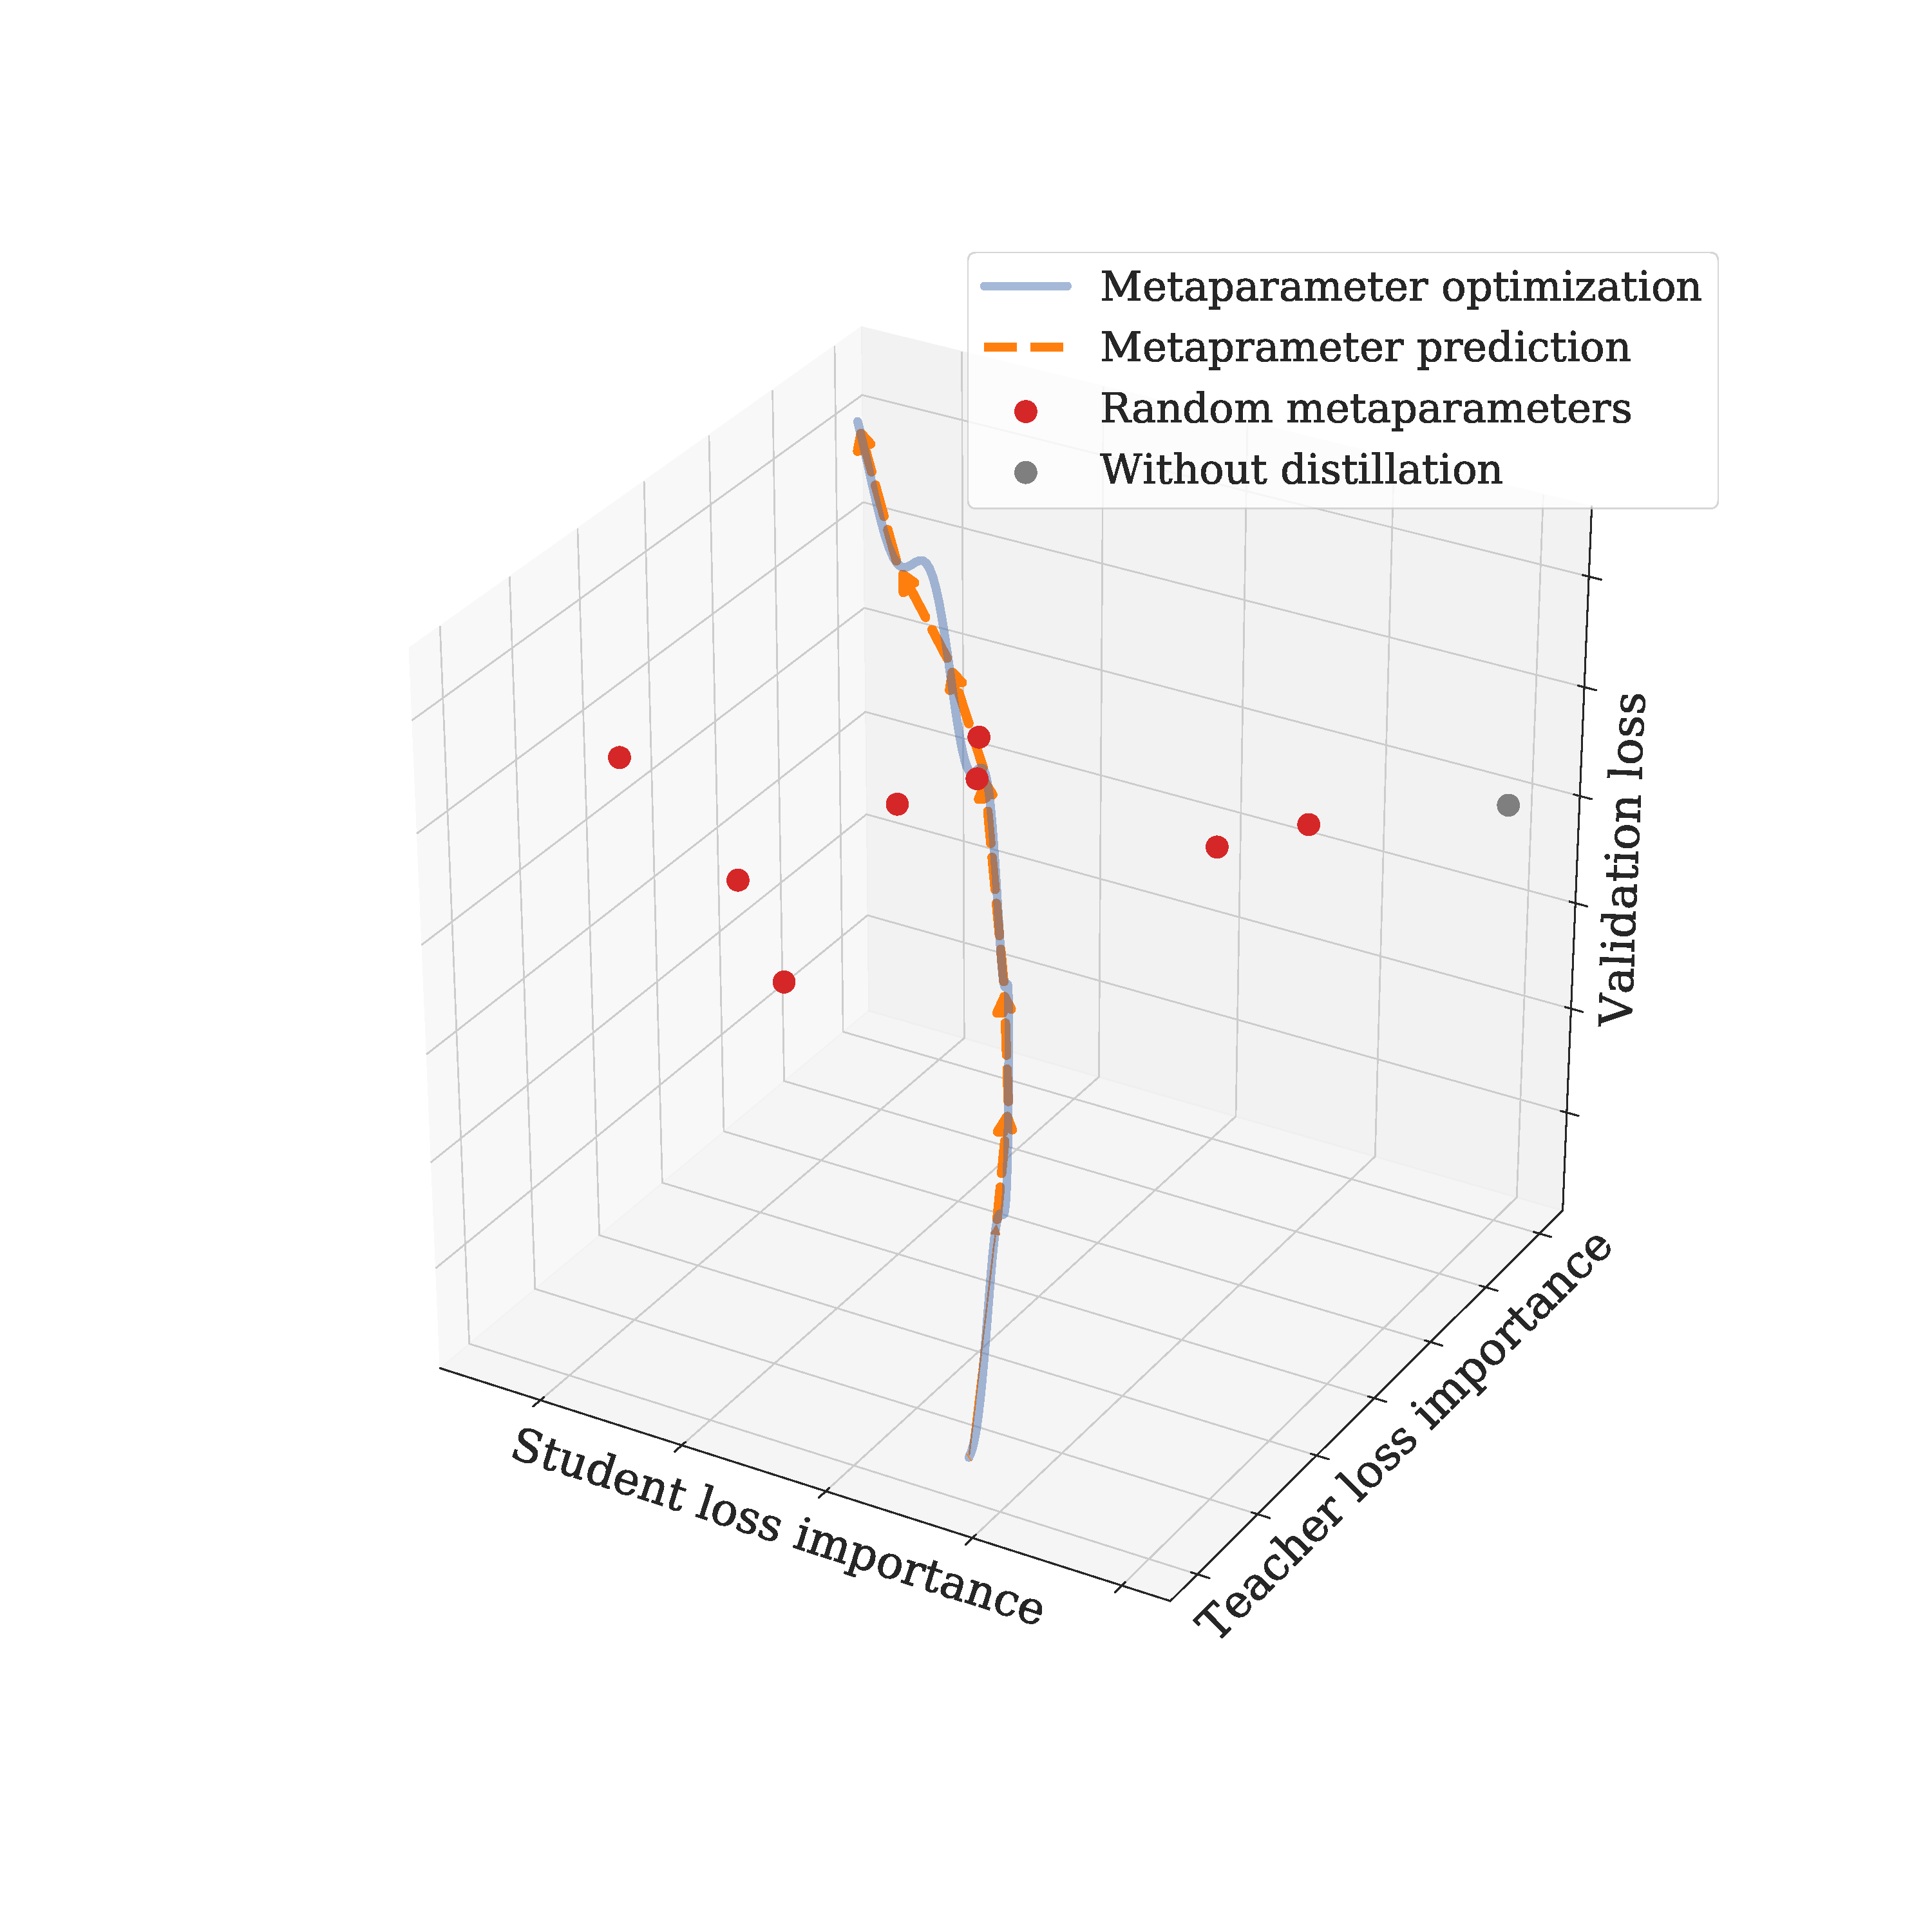
\includegraphics[width=0.7\linewidth]{trajectory.pdf}}
    \caption{A principle idea of the proposed method. The metaparameters control the final loss of the model. Instead of optimize the metaparameters straightforwardly we analyze the optimization trajectory and predict it using linear model.}
    \label{fig:trajectory}
\end{figure}

For the metaparameter optimization, we employ a bi-level optimization problem. Model parameters are optimized on the first level and the metaparameters are optimized on the second level. This approach is described in~\cite{journals/corr/LuketinaBR15,journals/anor/BakhteevS20,journals/corr/MaclaurinDA15}. The greedy gradient-based method  for the bi-level optimization problem is described in~\cite{journals/corr/LuketinaBR15}. In~\cite{journals/anor/BakhteevS20} different gradient-based algorithms and random search are analyzed. 
This paper analyzes the approach to optimizing and predicting metaparameters obtained after applying gradient-based methods. It can be seen from the Table~\ref{table:compl} that for the large-scale tasks the gradient-based methods of metaparameter optimization are more preferable. Nevertheless, the hyperparameter and metaparameters optimization still increases the model optimization time drastically~\cite{liu2018darts}. In order to decrease the optimization cost, we analyze the metaparameter optimization trajectory and predict it using linear model. The Fig. \ref{fig:trajectory} visualizes this approach. We evaluate our method and compare it with other metaparameter optimization methods on the image datasets CIFAR-10~\cite{krizhevsky2009learning}, Fashion-MNIST \cite{journals/corr/abs-1708-07747}, and synthetic dataset. 

Our contributions are:
\begin{enumerate}[{1)}]
    \item we compare two approaches for the metaparameter optimization for the knowledge distillation task: either stochastic and gradient-based;
    
    \item we propose a modification of the gradient-based optimization to reduce the computational cost of the optimization;
    
    \item we give a theoretical analysis for the proposed method and evaluate its performance for the knowledge distillation.
\end{enumerate}


\section{Problem statement}
There is given a dataset for $K$-classification problem:

$$
    \fD = \{(\bx_i, y_i)\}_{i=1}^{m},\; \bx_i \in \bbR^n,\; y_i \in \bbY = \{1, \dots, K\},
$$

\noindent
where $y_i$ is a class of $\bx_i$.

Split the dataset $\fD$: $\fD = \fD_\text{train} \sqcup \fD_\text{val}.$ The subset $\fD_\text{train}$ is used for model parameter optimization, the subset $\fD_\text{val}$ for metaparameter optimization.

Given a teacher model $\bff$, which was trained on the dataset $\fD_\text{train}$. Optimize a student model $\bg$ to transfer information obtained from  the teacher. The following definition gives a formal statement for this problem.

\begin{definition}
Let function~$D: \bbR^s \to \bbR_{+}$ defines the distance between the student model~$\bg$ and the teacher model~$\bff$. $D$-distillation of a student model is a student model parameter optimization problem that minimizes the function~$D$.
\end{definition}

Construct the $\cL_\text{train}$ loss function that takes into account the knowledge distillation from model $\bff$ to model $\bg$:

\begin{multline*}
    \cL_\text{train}(\bw, \boldsymbol{\lambda}) = -\lambda_1\sum\limits_{(\bx, y) \in \fD_\text{train}}\underbrace{\sum\limits_{k=1}^{K}y^k\log \frac{e^{\bg(\bx, \bw)_k}}{\sum\limits_{j=1}^{K}e^{\bg(\bx, \bw)_j}}}_{\text{classification term}} \\- (1 - \lambda_1)\sum\limits_{(\bx, y) \in \fD_\text{train}}\underbrace{\sum\limits_{k=1}^{K}\frac{e^{\bff(\bx)_k/T}}{\sum\limits_{j=1}^{K}e^{\bff(\bx)_j/T}}\log \frac{e^{\bg(\bx, \bw)_k/T}}{\sum\limits_{j=1}^{K}e^{\bg(\bx, \bw)_j/T}}}_{\text{distillation term}},
\end{multline*}

\noindent
where~$y_k$ is the $k$-th component of the target vector,~$T$ is a temperature in the distillation problem. The temperature $T$ has the following properties:

\begin{enumerate}[{1)}]
    \item when $T \rightarrow 0$ we obtain a vector that has one class with unit probability;
    \item when $T \rightarrow \infty$ we obtain the classes with equal probability.
\end{enumerate}

\begin{lemma}
When~$\lambda_1 = 0$ we minimize loss function which is a $D$-distillation with $D = D_{KL}\left(\sigma\left(\bff/T\right), \sigma\left(\bg/T\right)\right)$, where $\sigma$ is a softmax function.
\end{lemma}

\begin{proof}
When~$\lambda_1 = 0$ we have:

\begin{multline*}
    \cL_\text{train}(\bw, \boldsymbol{\lambda}) = \sum\limits_{(\bx, y) \in \fD_\text{train}}\sum\limits_{k=1}^{K}\frac{e^{\bff(\bx)_k/T}}{\sum\limits_{j=1}^{K}e^{\bff(\bx)_j/T}}\log \frac{e^{\bg(\bx, \bw)_k/T}}{\sum\limits_{j=1}^{K}e^{\bg(\bx, \bw)_j/T}} \\= D_{KL}\left(\sigma(\bff(\bx)/T), \sigma(\bg(\bx, \bw)/T)\right).
\end{multline*}

The function $D_{KL}\left(\sigma\left(\bff/T\right), \sigma\left(\bg/T\right)\right)$ defines the distance between logits of model $\bff$ and model $\bg$. Therefore, the definition of the $D$-distillation is satisfied. \qed

\end{proof}

% $\hspace{12.3 cm}\Box$

Define the set of metaparameters~$\boldsymbol{\lambda}$ as a vector which components are coefficients before terms of $\cL_\text{train}$ and temperature~$T$:

\[\boldsymbol{\lambda} = [\lambda_1, T].\]
Define the bi-level optimization problem:
\begin{equation} \label{eq:opt_hyp}
    \hat{\boldsymbol{\lambda}} = \arg\min\limits_{\boldsymbol{\lambda} \in \bbR^2} \cL_\text{val}(\hat{\bw}, \boldsymbol{\lambda}),
\end{equation}
\begin{equation} \label{eq:opt_param}
    \hat{\bw} = \arg\min\limits_{\bw \in \bbR^s} \cL_\text{train}(\bw, \boldsymbol{\lambda}),
\end{equation}
where $\cL_\text{val}$ is a validation loss function:

$$
     \cL_\text{val}(\bw, \boldsymbol{\lambda}) = - \sum\limits_{(\bx, y) \in \fD_\text{val}}\sum\limits_{k=1}^{K}y^k\log \frac{e^{\bg(\bx, \bw)_k/T_\text{val}}}{\sum\limits_{j=1}^Ke^{\bg(\bx, \bw)_j/T_\text{val}}},
$$
the metaparameter $T_\text{val}$ controls the temperature for the validation loss. It is set manually and is not subject to optimization. 
% \section{Gradient-based methods}
\section{Gradient-based metaparameter optimization}
One of the methods to  optimize metaparameters is to use a gradient-based method. Below we describe the scheme of its usage and an approach to approximate the trajectory of the optimized metaparameters.

\begin{definition} 
Define an \textit{optimization operator} as an algorithm $U$ that selects the model parameter vector $\bw^\prime$ using the parameters on the previous step $\bw$.
\end{definition}

Optimize the parameters $\bw$ using $\eta$ optimization steps:

$$
    \hat{\bw} = U \circ U \circ \dots \circ U(\bw_0, \boldsymbol{\lambda}) = U^\eta(\bw_0, \boldsymbol{\lambda}),
$$

\noindent
where $\bw_0$ is the initial value of the model parameter vector $\bw$, $\boldsymbol{\lambda}$ is the set of metaparameters.

Redefine the optimization problem using the operator $U$:

$$
    \hat{\boldsymbol{\lambda}} = \arg\min\limits_{\boldsymbol{\lambda} \in \bbR^2} \cL_\text{val}\bigl(U^\eta(\bw_0, \boldsymbol{\lambda})\bigr).
$$

%The scheme of metaparameter optimization is the following: 
%\begin{enumerate}
%     \item In range from $1$ to $l$, where $l$ is the number of the metaparameter optimization iterations:
%     \item Solve the problem \eqref{eq:hyp_oper} and obtain the new metaparameter value $\boldsymbol{\lambda}^\prime$.
%     \item Let $\boldsymbol{\lambda} = \boldsymbol{\lambda}^\prime$,
% \end{enumerate}
% where $l$ is the number of the metaparameter optimization iterations. 
Solve optimization problem \eqref{eq:opt_hyp} and \eqref{eq:opt_param} with gradient descent operator:
$$
    U(\bw, \boldsymbol{\lambda}) = \bw - \gamma\nabla\cL_\text{train}(\bw, \boldsymbol{\lambda}),
$$
where $\gamma$ is a learning rate. For the metaparameter optimization we use the greedy gradient-based method, which depends only on the model parameter value $\bw$ on the previous step. On every iteration we obtain the following metaparameter value:
\begin{equation}
    \boldsymbol{\lambda}^\prime = \boldsymbol{\lambda} - \gamma_{\boldsymbol{\lambda}}\nabla_{\boldsymbol{\lambda}}\cL_\text{val}(U(\bw, \boldsymbol{\lambda}), \boldsymbol{\lambda}) = \boldsymbol{\lambda}\\ - \gamma_{\boldsymbol{\lambda}}\nabla_{\boldsymbol{\lambda}}\cL_\text{val}(\bw - \gamma\nabla\cL_\text{train}(\bw, \boldsymbol{\lambda}), \boldsymbol{\lambda}).
    \label{eq:hyp_alg}
\end{equation}
In this paper we use a numerical difference approximation for this optimization procedure~\cite{liu2018darts}. For further optimization cost reduction we propose to approximate the metaparameter optimization path. The path is predicted with linear models that are used periodically after a certain number of iterations  $e_1$. After that the linear model is used to predict metaparameters for $e_2$ iterations:
\begin{equation}
     \boldsymbol{\lambda}^\prime = 
     \boldsymbol{\lambda} + \bc^{\top}\begin{pmatrix}z\\1\end{pmatrix},
     \label{eq:linear}
\end{equation}
where $\mathbf{c}$ is the vector of parameters optimized using least squares method, $z$ is a number of optimization iteration. The algorithm of the proposed method is show in Fig.~\ref{algo}.

%-------Algorithm----
\begin{figure}
\begin{algorithm}[H]
\caption{Metaparameter optimization}
 \begin{algorithmic}[1]

 %\renewcommand{\algorithmicrequire}{\mathbf{Input:}}
 %\renewcommand{\algorithmicensure}{\mathbf{Output:}}
 \REQUIRE number $e_1$ of iterations to use gradient-based optimization 
 \REQUIRE number $e_2$ of iterations to use linear predictions for metaparameters $\boldsymbol{\lambda}$  
 %\REQUIRE in
 %\ENSURE  out
  \WHILE {not converged}
  \STATE Optimize $\boldsymbol{\lambda}$ and $\mathbf{w}$ for $e_1$ iterations solving a bi-level optimization problem
  \STATE $\textbf{traj} = $trajectory of $(\nabla \boldsymbol{\lambda})$ changes during optimization;
  \STATE Set $\mathbf{z} = [1,\dots,e_1]^\mathsf{T}$
  \STATE Optimize $\mathbf{c}$ using least square method: 
  $$\hat{\mathbf{c}} = \argmin_{\mathbf{c} \in \mathbb{R}^2} ||\textbf{traj} - \mathbf{z}\cdot c_1 + c_2||_2^2$$
  \STATE Optimize $\mathbf{w}$ and predict $\boldsymbol{\lambda}$ for $e_2$ iterations using linear model with parameters $\mathbf{c}$.
  \ENDWHILE

 \end{algorithmic}
 \end{algorithm}
 \caption{An algorithm for the proposed method.}
 \label{algo}

 \end{figure}
 
%In this algorithm $z$ is a remainder of iteration number divided by the period $e_2$ of linear model training, $\bc$ is a vector of linear model parameters. We optimize the parameters $\bc$ using least squares method periodically with a pre-defined $p$. The value of $e_2$ is tuned during cross-validation procedure. $G$ is a set of gradients, $e_1$ is a number of iterations in one epoch.

%\vspace{0.7 cm}
% \begin{equation*}
% \xymatrix{
% (-\lambda^2\nabla_{\textbf{w}}S+\textbf{w})\ar[r]^{\qquad T} & \hat{\textbf{w}}, \textbf{x} \ar[r]^f &  \hat{y}\ar[r] & S(\mathbf{\textbf{w}|y,\hat{y}}) \ar@/_3pc/[lll]\\
% %1 & 2 &  & y\ar[ur] & 5 \\
% t\ar[r] & i\ar[r] & (\textbf{x}, y)\ar[ul]\ar[ur] & }
% \end{equation*}

The diagram on Fig.~\ref{fig:scheme} presents resulting optimization method. Model parameters are optimized on the first level of a bi-level optimization problem using $\fD_\text{train}$ subset and $\cL_{\text{train}}$ function. Metaparameters are optimized in the second level using $\fD_\text{val}$ subset and $\cL_\text{val}$ function. During $e_1$ iterations metaparameters are optimized using SGD and during $e_2$ iterations they are predicted using linear model. Then the obtained metaparameter values are used for model parameter optimization.
\begin{figure}
$$
\xymatrix{
\bw - \gamma\nabla\cL_\text{train}(\bw, \boldsymbol{\lambda})\ar[r] & \hat{\bw}, \bx\ar[r]^{\bg} & \hat{y}\ar[r] & \cL_\text{train}(\bw, \boldsymbol{\lambda})\ar@/_2pc/[lll]\\
t\ar[r] & i\ar[r] & (\bx, \by)\ar[r]\ar[dr] & \fD_\text{train}\ar[u]\\
 &  &  & \fD_\text{val}\ar[d]_{e_1}\\
 &  &  & \cL_{\text{val}}(\boldsymbol{\lambda})\ar[dll]\\
 & \boldsymbol{\lambda} - \gamma_{\boldsymbol{\lambda}}\nabla_{\boldsymbol{\lambda}}\cL_\text{val}(U(\bw, \boldsymbol{\lambda}), \boldsymbol{\lambda})\ar[rr] &  & \boldsymbol{\lambda}^\prime\ar[u]\ar@/_0.5pc/[d]_{e_2}\ar@/_2pc/[uuuu]\\
 &  &  & \boldsymbol{\lambda}^\prime + \bc^\T\textbf{z}\ar@/_0.5pc/[u]
}
$$
\caption{The diagram for the metaparameters optimization.}
\label{fig:scheme}

\end{figure}

% \begin{itemize}
% \item[] $f$ is the forecasting model,
% \item[] $S$ is the criterion,
% \item[] $T$ is an optimization algorithm,
% \item[] $\hat{\textbf{w}}$ is some solution,
% \end{itemize}

% \begin{equation*}
% \hat{\textbf{w}}= \arg\min S(\textbf{w}|y,f).
% \end{equation*}

\noindent
The following theorem proves the correctness of the  approximation by a linear model.

\begin{theorem}
If function $\mathcal{L}_{\textnormal{train}}(\bw, \boldsymbol{\lambda})$ is smooth and convex and its Hessian $\mathbf{H} = \nabla_{\bw}^2 \mathcal{L}_\textnormal{train}$  is invertible and can be well approximated by identity, $\mathbf{H} \approx \mathbf{I},$ then greedy algorithm~\eqref{eq:hyp_alg} finds optimum solution of the bi-level problem \eqref{eq:opt_hyp}. If there is a domain $\cD \in \bbR^2$ in metaparameter space where the gradient of metaparameters can be well approximated by a constant, then the optimization is linear w.r.t the metaparameters.
\end{theorem}

\begin{proof} 
In work \cite{journals/corr/Pedregosa16} it was derived a formula for $\nabla_{\boldsymbol{\lambda}}\mathcal{L}_\text{val} = \nabla_{\boldsymbol{\lambda}}\mathcal{L}_\text{val}(U(\bw, \boldsymbol{\lambda}))$ in case when $\mathcal{L}_\text{train}(\textbf{w}, \boldsymbol{\lambda})$  is smooth and convex and $\mathbf{H}$ is invertible:

$$
    \nabla_{\boldsymbol{\lambda}}\mathcal{L}_\text{val}(\boldsymbol{\lambda}) = \nabla_{\boldsymbol{\lambda}}\mathcal{L}_\text{val} - (\nabla_{\textbf{w}, \boldsymbol{\lambda}}^2\mathcal{L}_\text{train})^\top(\nabla_{\textbf{w}}^2\mathcal{L}_\text{train})^{-1}\nabla_{\textbf{w}}\mathcal{L}_\text{val}.
$$

It can be simplified by excluding the first term because function $\mathcal{L}_\text{val}$ does not depend on metaparameters explicitly:

$$
    \nabla_{\boldsymbol{\lambda}}\mathcal{L}_\text{val}(\boldsymbol{\lambda}) = - (\nabla_{\textbf{w}, \boldsymbol{\lambda}}^2\mathcal{L}_\text{train})^\top(\nabla_{\textbf{w}}^2\mathcal{L}_\text{train})^{-1}\nabla_{\textbf{w}}\mathcal{L}_\text{val}.
$$

If $\nabla_{\textbf{w}}^2 \mathcal{L}_\text{train}$ can be well approximated by identity then greedy algorithm gives optimum to the bi-level problem if its step has the following formula~\cite{journals/corr/LuketinaBR15}:

$$
    \boldsymbol{\lambda}_{t+1} = \boldsymbol{\lambda}_{t} + \eta_1(\nabla_{\textbf{w}, \boldsymbol{\lambda}}^2\mathcal{L}_\text{train})^\top\nabla_{\textbf{w}}\mathcal{L}_\text{val}.
$$

We also exclude $\nabla_{\textbf{w}}^2 \mathcal{L}_\text{train}$  by replacing it with identity.

Return to the simplified formula of the gradient:

$$\nabla_{\boldsymbol{\lambda}}\mathcal{L}_\text{val}(\boldsymbol{\lambda}) = - (\nabla_{\textbf{w}, \boldsymbol{\lambda}}^2\mathcal{L}_\text{train})^\top\nabla_{\textbf{w}}\mathcal{L}_\text{val}.$$

Suppose that there is a domain $\cD$ where $\nabla_{\boldsymbol{\lambda}}\mathcal{L}_\text{val}(\boldsymbol{\lambda})$ can be approximated by a constant vector

\[\nabla_{\boldsymbol{\lambda}}\mathcal{L}_\text{val}(\boldsymbol{\lambda}) \approx \begin{pmatrix} a_1\\ a_2\end{pmatrix}.\]

Then on $\cD$ the optimization  step can be represented as
$$
    \boldsymbol{\lambda}_{t+1} = \boldsymbol{\lambda}_{t} - \gamma_{\boldsymbol{\lambda}}\begin{pmatrix} a_1\\ a_2\end{pmatrix},
$$
\noindent
which has a linear form similar to~\eqref{eq:linear}. \qed
\end{proof}

\section{Experiments}
The purpose of the experiment is to evaluate the performance of the proposed distillation method and to analyze the resulting models and their metaparameters. The method is evaluated using the synthetic dataset, Fashion-MNIST dataset, and CIFAR-10 dataset.~\footnote{The source code for the computational experiment will be available in the camera-ready version of the paper.} For the CIFAR-10, we conducted two experiments: on the whole dataset and the reduced training subset, $|\mathfrak{D}_\text{train}|=12800$. 


We analyzed the following metparameter optimization methods:
\begin{enumerate}[{1)}]
    \item optimization without distillation;
    \item optimization with randomly initialized metaparameter values. The metaparameters were sampled from uniform distribution $$\lambda_1 \sim \mathcal{U}(0;1), \quad T \sim \mathcal{U}(0.1, 10).$$
    \item optimization with ``naive'' metaparameter assignment: setting $$\lambda_1 = 0.5, T = 1;$$
    \item gradient-based optimization;
    \item proposed method with $e_1=e_2=10$.
\end{enumerate}

We used a full training dataset $\fD$ for the methods 1-3. For all the experiments except the experiment on the full  CIFAR-10 dataset we also used metaparameter optimization with probablistic model. As a such optimization we used hyperopt library~\cite{bergstra2013making} providing a Parzen estimator-based metparameter optimization. For this method we used 5 run before the final metaparameter prediction.

We used accuracy as an external criterion:
$$
    \text{accuracy} = \frac{1}{m}\sum\limits_{i=1}^m [\bg(\bx_i, \bw) = y_i],
$$
For all the experiment we sample initial metaparameter values in the following way: 
$$\lambda_1 \sim \mathcal{U}(0,1),\quad \log_{10} T \sim \mathcal{U}(-1, 1).$$ All the experiments were ran 10 times, the results were averaged. 

The overall results are displayed in Table~\ref{table:results}. The dependency of the accuracy on the epoch number for the synthetic dataset and reduced CIFAR-10 dataset is shown in Fig.~\ref{fig:accuracy}.

\begin{table}[]

\caption{Experiment results. The numbers in brackets correspond to the maximum values in the experiment. }

\label{table:results}
\footnotesize
\centering
\begin{tabularx}{\textwidth}{|X|X|X|X|X|X}
\cline{1-5}
Method                      & Synthetic dataset & Fashion-MNIST & Reduced CIFAR-10 & CIFAR-10      &  \\ \cline{1-5}
Without distillation        & 0.63 (0.63)             & 0.87  (0.88)        & 0.55     (0.56)        & 0.65 (0.66)         &  \\ \cline{1-5}
Naive metaparameters        & 0.63  (0.63)              & 0.87 (0.88)         & 0.55  (0.56)             & 0.66  (0.67)        &  \\ \cline{1-5}
Random metaparameters       & 0.64   (0.72)           & 0.79   (0.88)       & 0.54 (0.57)             & 0.64 (0.67)        &  \\ \cline{1-5}
Gradient-based optimization & \textbf{0.77} (0.78)    & \textbf{0.88} (0.89) & \textbf{0.57} (0.61)    & \textbf{0.70} (0.72) &  \\ \cline{1-5}
Hyperopt                    & \textbf{0.77} (0.78)                & 0.87 (0.88)         & 0.55  (0.58)           & -             &  \\ \cline{1-5}
Proposed                    & 0.76   (0.78)           & \textbf{0.88} (0.89) & \textbf{0.57}    & \textbf{0.70} (0.72) &  \\ \cline{1-5}
\end{tabularx}
\end{table}

\begin{figure}[ht]
    \begin{subfigure}[h]{0.5\linewidth}
    \center{
    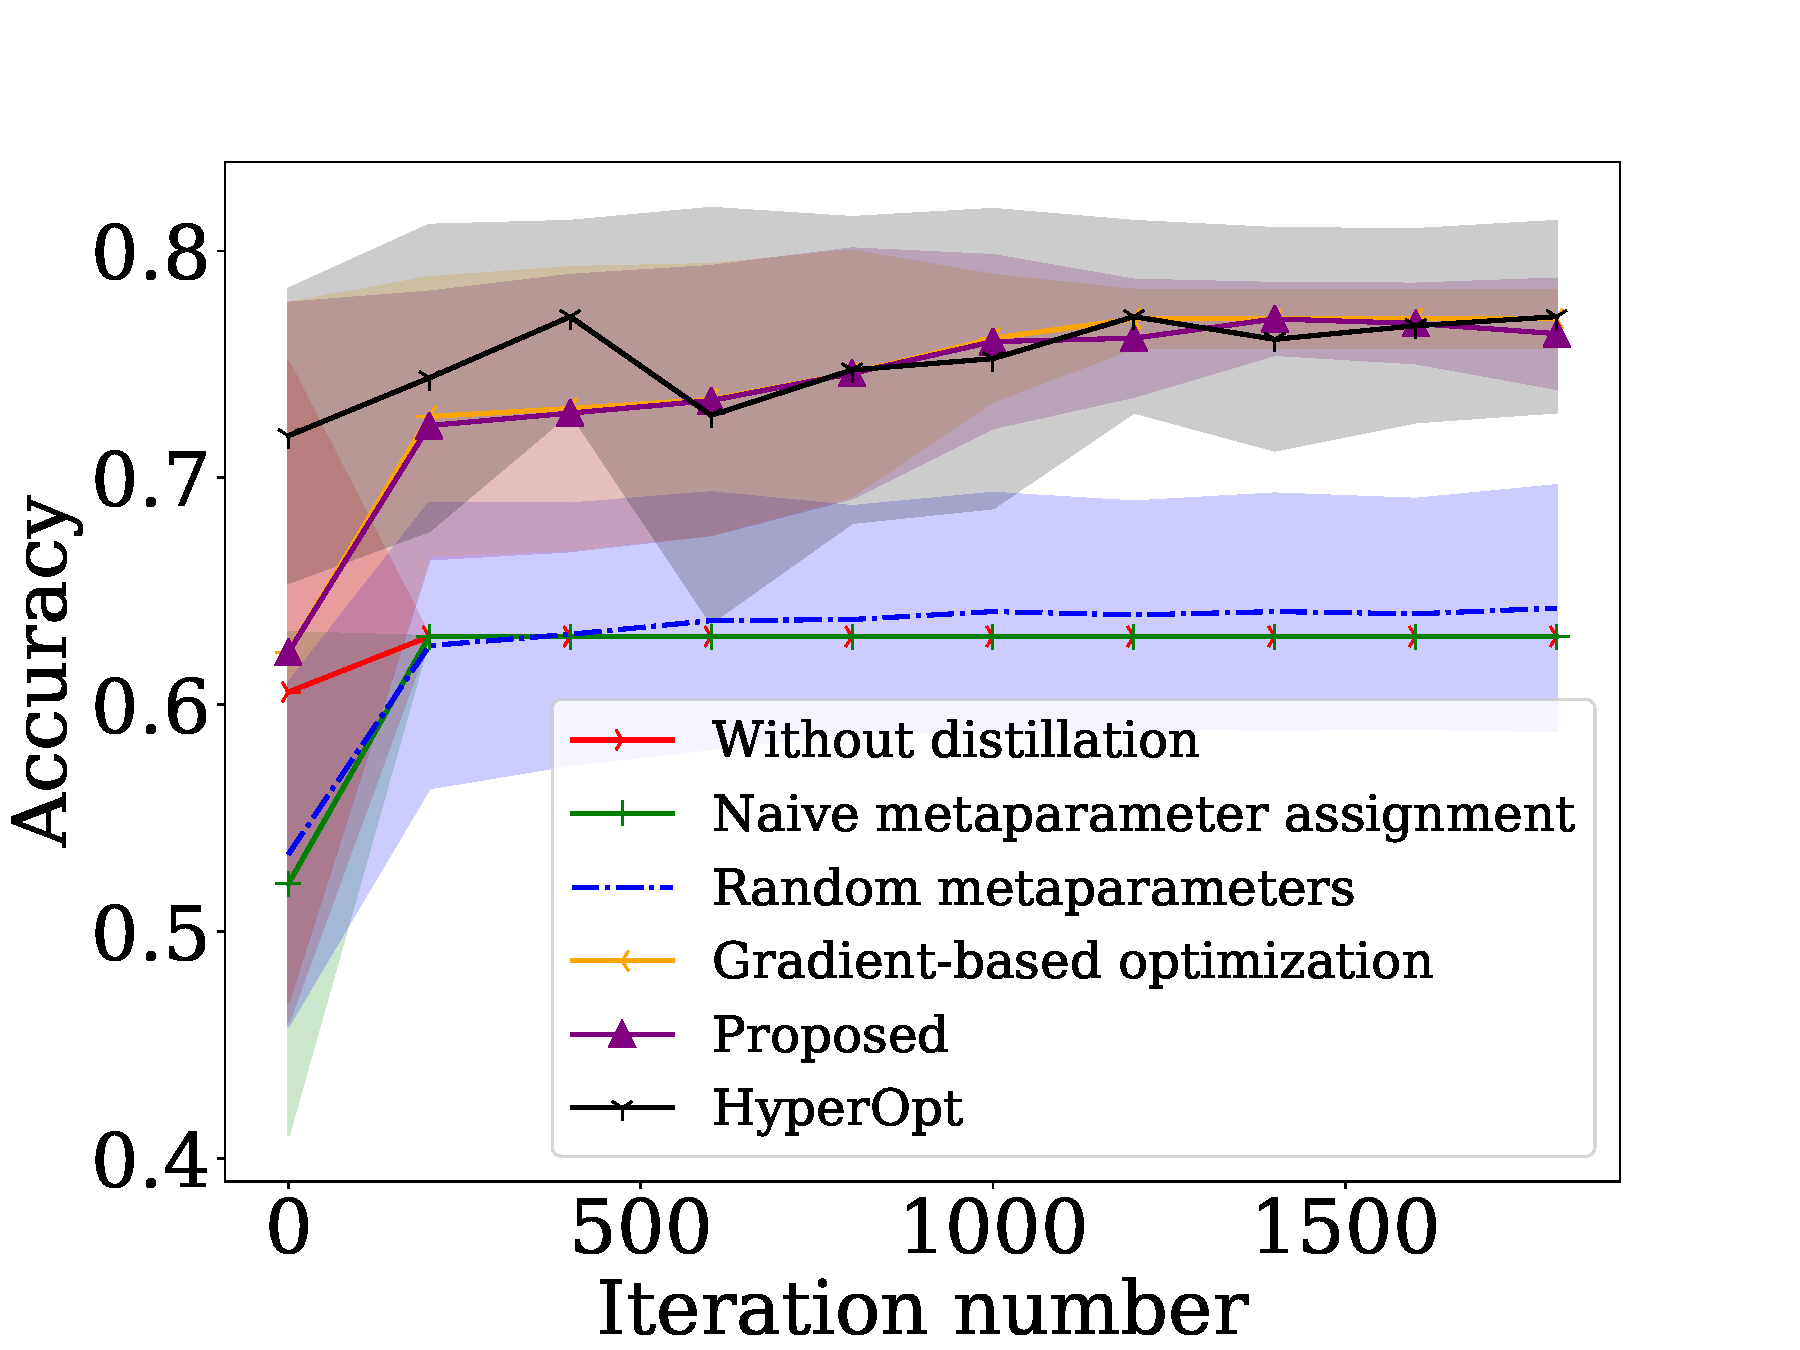
\includegraphics[width=\linewidth]{synth_accuracy.pdf}}
    \caption{}
    \label{fig:epoch_size}
    \end{subfigure}
    \begin{subfigure}[h]{0.5\linewidth}
    \center{
    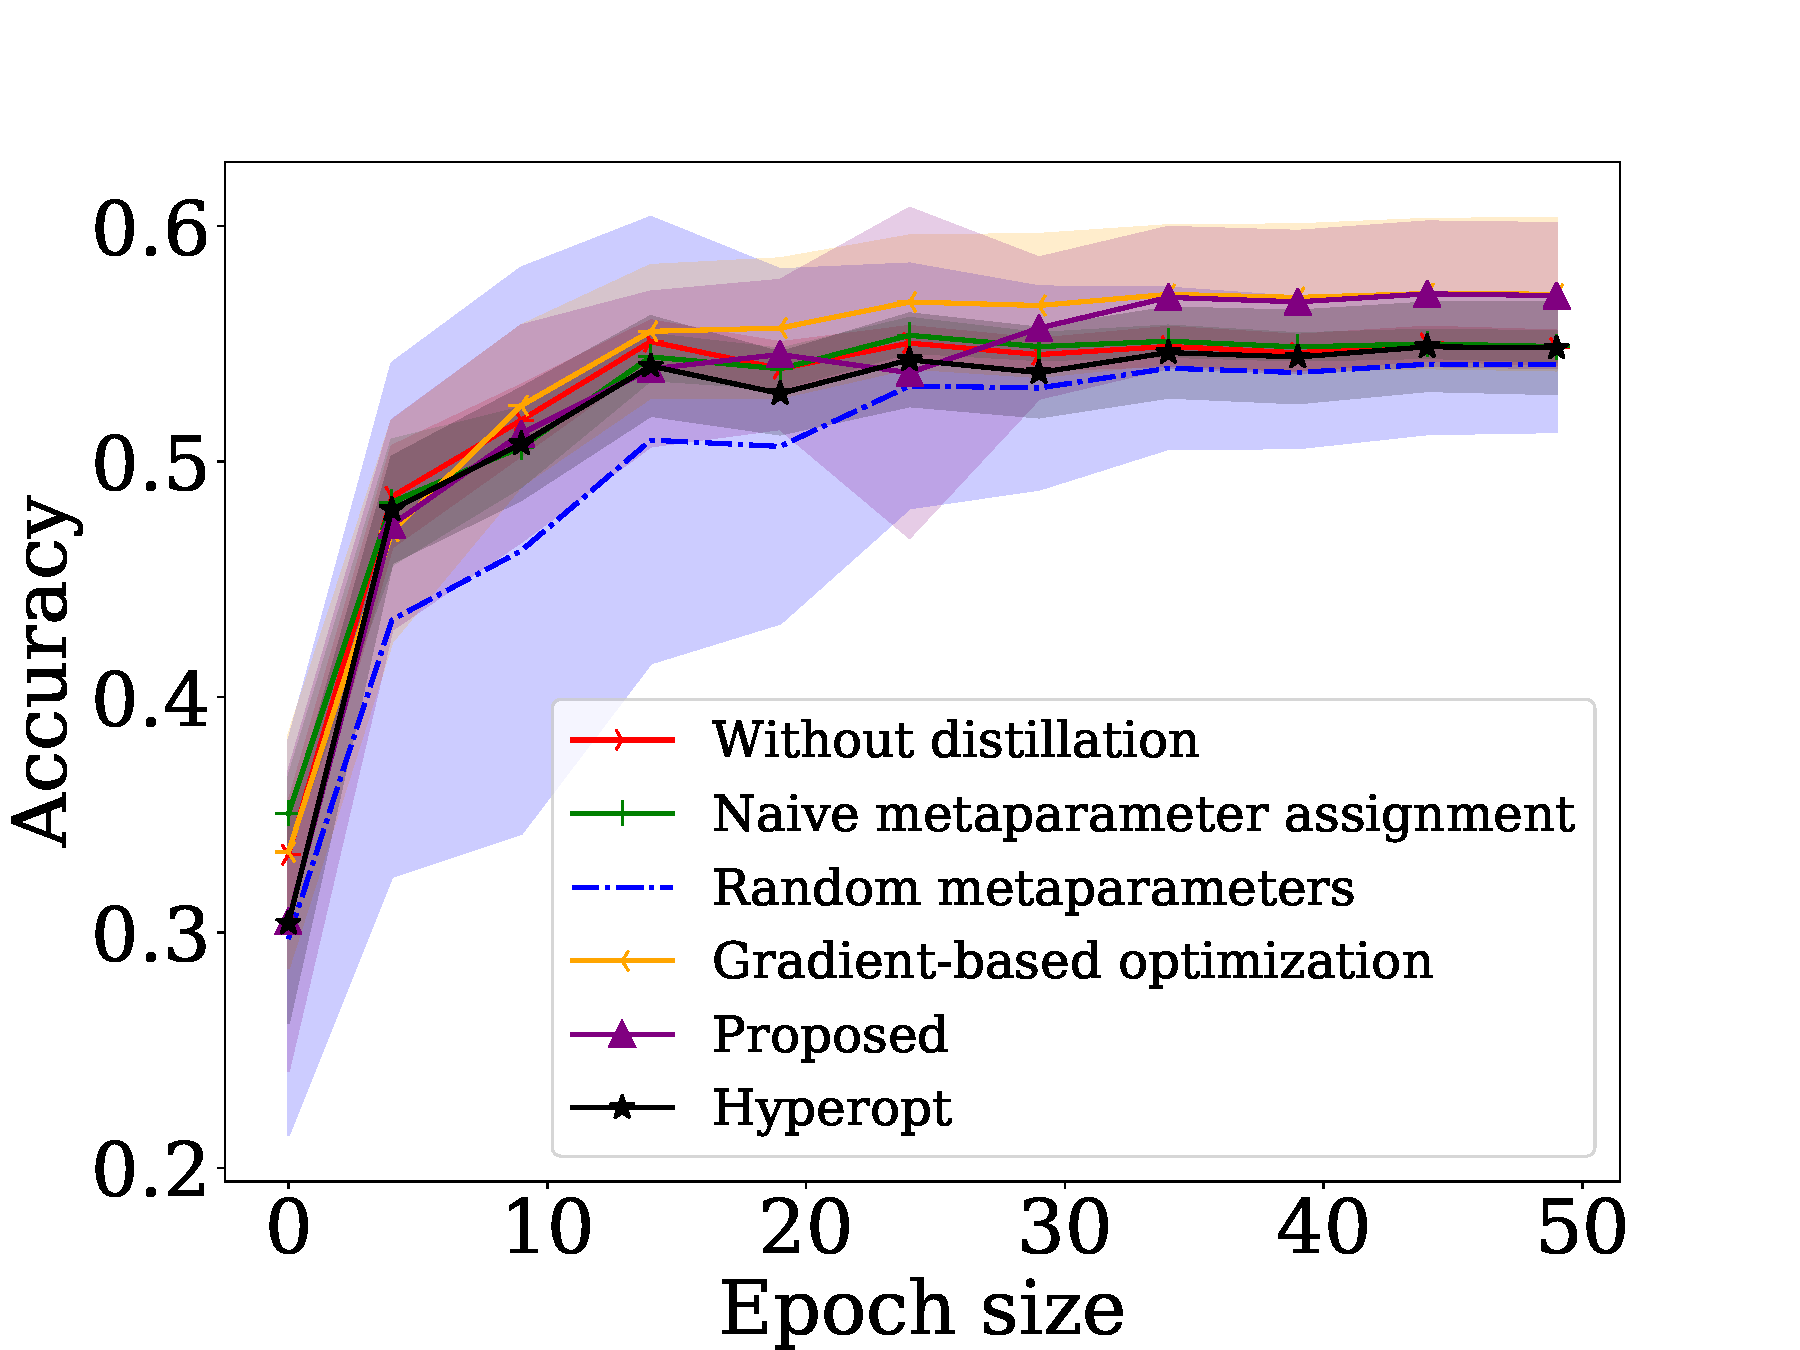
\includegraphics[width=\textwidth]{mini_cifar_accuracy.pdf}}
    \caption{}
    \label{fig:train_splines_every_epoch}
    \end{subfigure}
    % \vspace{-0.2 cm}
    \caption{%\fontsize{10}{5}\selectfont
    Model accuracy for different datasets: a) syntetic dataset, b) CIFAR-10 reduced dataset.}
    \label{fig:accuracy}
\end{figure}
 
 
\subsection{Experiment on synthetic dataset}
For the evaluation of the method we conducted a computational experiment using a synthetic dataset:
\begin{gather*}
    \fD = \{(\bx_i, y_i)\}_{i=1}^{m}, \quad x_{ij} \in \cN(0, 1),\; j=1, 2, \quad x_{i3} = [\text{sign}(x_{i1})+\text{sign}(x_{i2})>0],\\
    y_i = \text{sign}(x_{i1}\cdot x_{i2}+\delta),
\end{gather*}
where~$\delta \in \cN(0, 0.5)$ is a noise. The size of the student model dataset is much smaller than the size of the teacher model dataset and $\fD_\text{train}$. In order to show the proof of concept for the proposed method, in this experiment, we split the dataset into 3 parts: the training dataset for the teacher, consisting of 200 objects, the training dataset for the student, consisting of 15 objects, and the validation part, which equals to the test dataset, $\fD_\text{val} = \fD_\text{test}$. It also consists of 200 objects. The visualization of the synthesized dataset is shown in Fig.~\ref{fig:synth}. The teacher was trained for 20000 iterations SGD with a learning rate equal to $10^{-2}.$ For its training, we used modified feature space:
\[
    x_{i3} = [\text{sign}(x_{i1})+\text{sign}(x_{i2}) + 0.1 >0].
\]
The purpose of such  modification is to prevent the teacher from nearly perfect fitting on the training dataset. In this case, learning without classification term, $\lambda_1 = 0$, would be preferable for the student.   The student model was trained for 2000 iterations with SGD learning rate equal to 1.0 and $T_\text{val} = 0.1.$

There were conducted series of experiments to determine the best $e_1$ and the best $e_2$. Fig. \ref{fig:epoch_size}.a plots the model accuracy for different $e_1$ with $e_2$ set to 10. Fig. \ref{fig:epoch_size}.b plots the model accuracy for different $e_2$. As we can see, with increasing $e_1$ and $e_2$ the approximation quality of metaparameter update trajectory  decreases.

\begin{figure}[ht]
    % \fontsize{5}{5}\selectfont
    \begin{subfigure}[h]{0.325\linewidth}
    \center{
    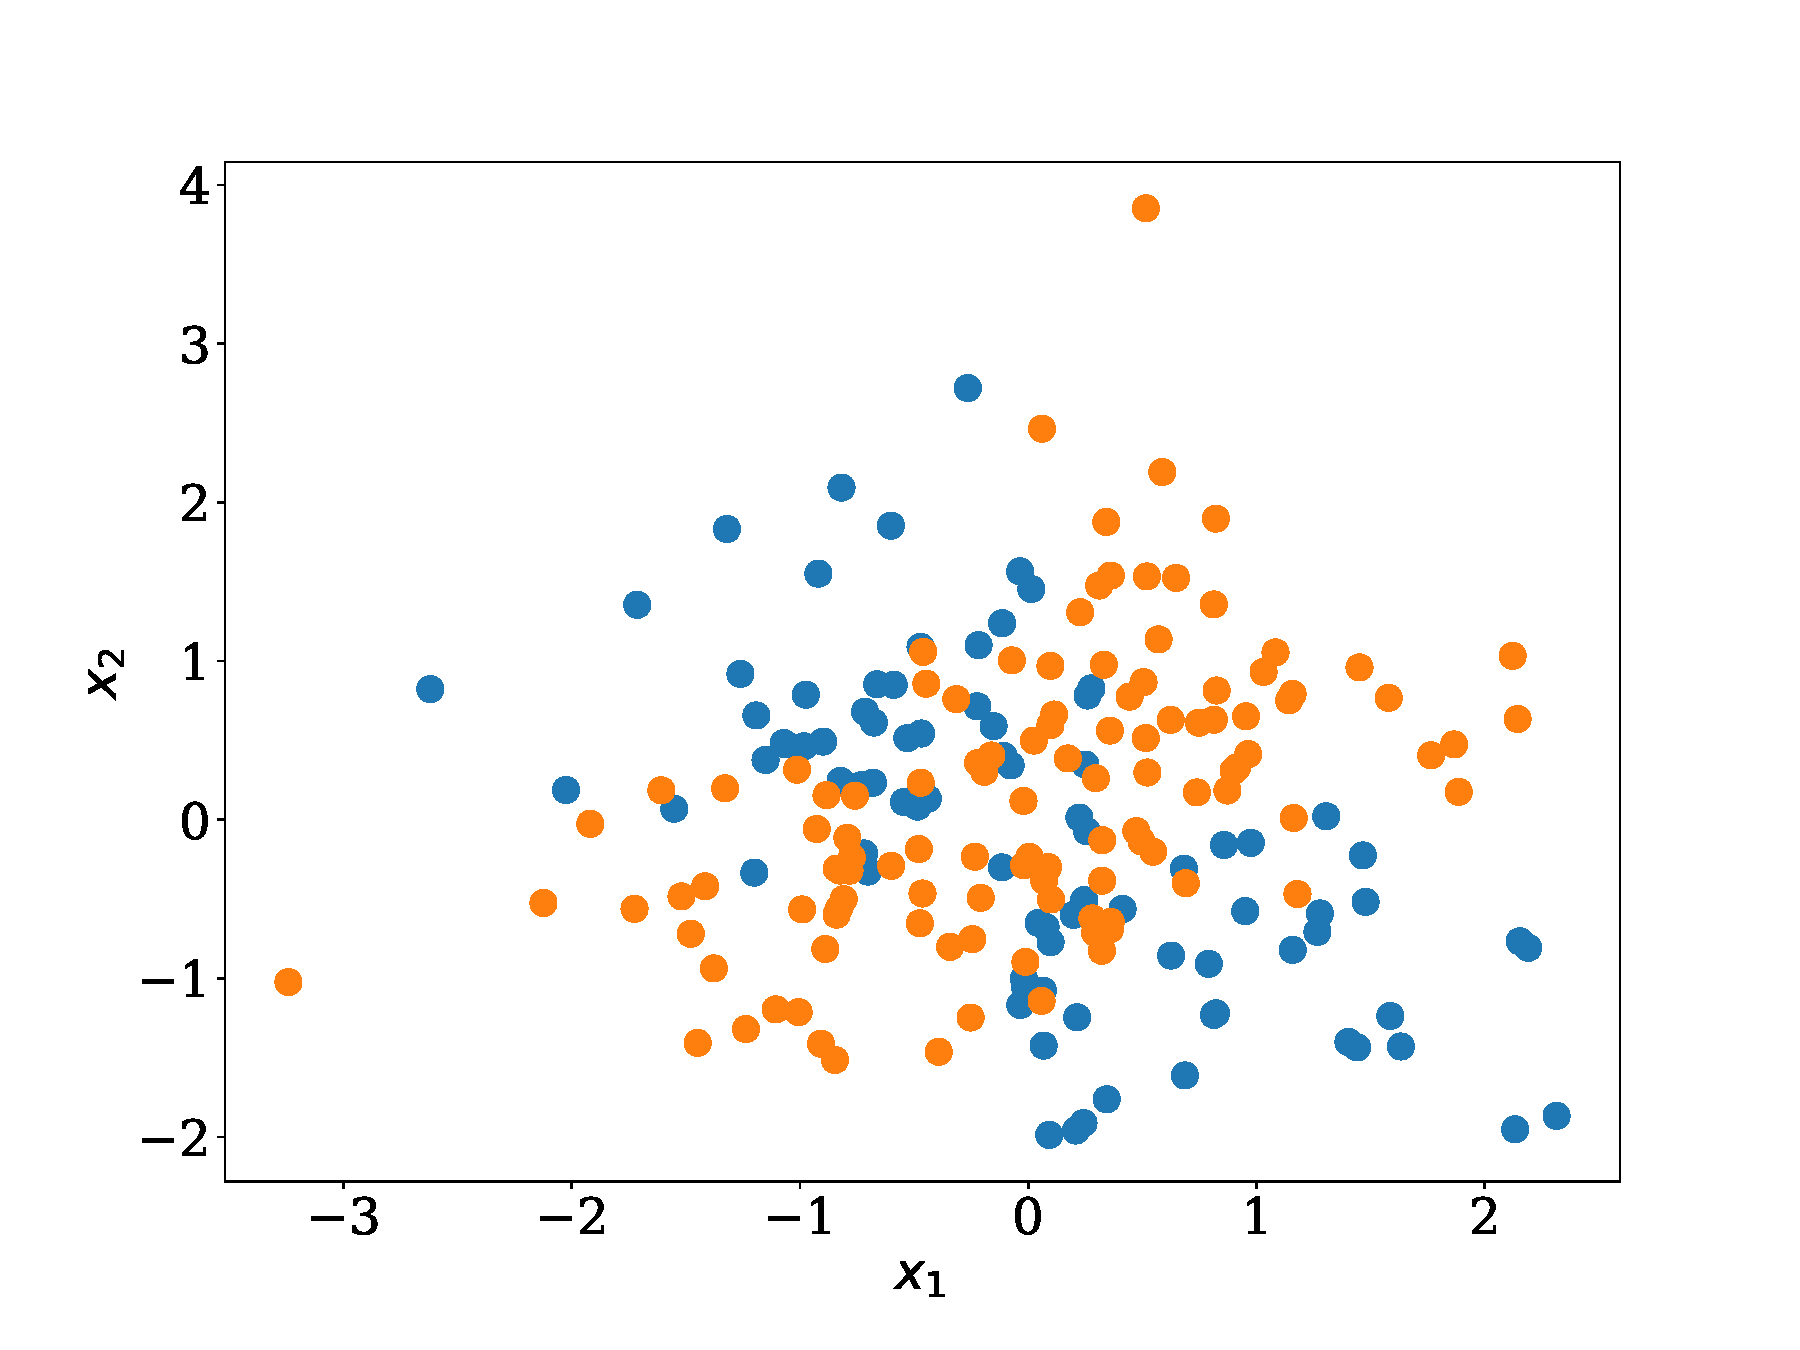
\includegraphics[width=\linewidth]{ttrain.pdf}
    \caption{}}
    \end{subfigure}
    % \hspace{-0.2cm}
    \begin{subfigure}[h]{0.325\linewidth}
    \center{
    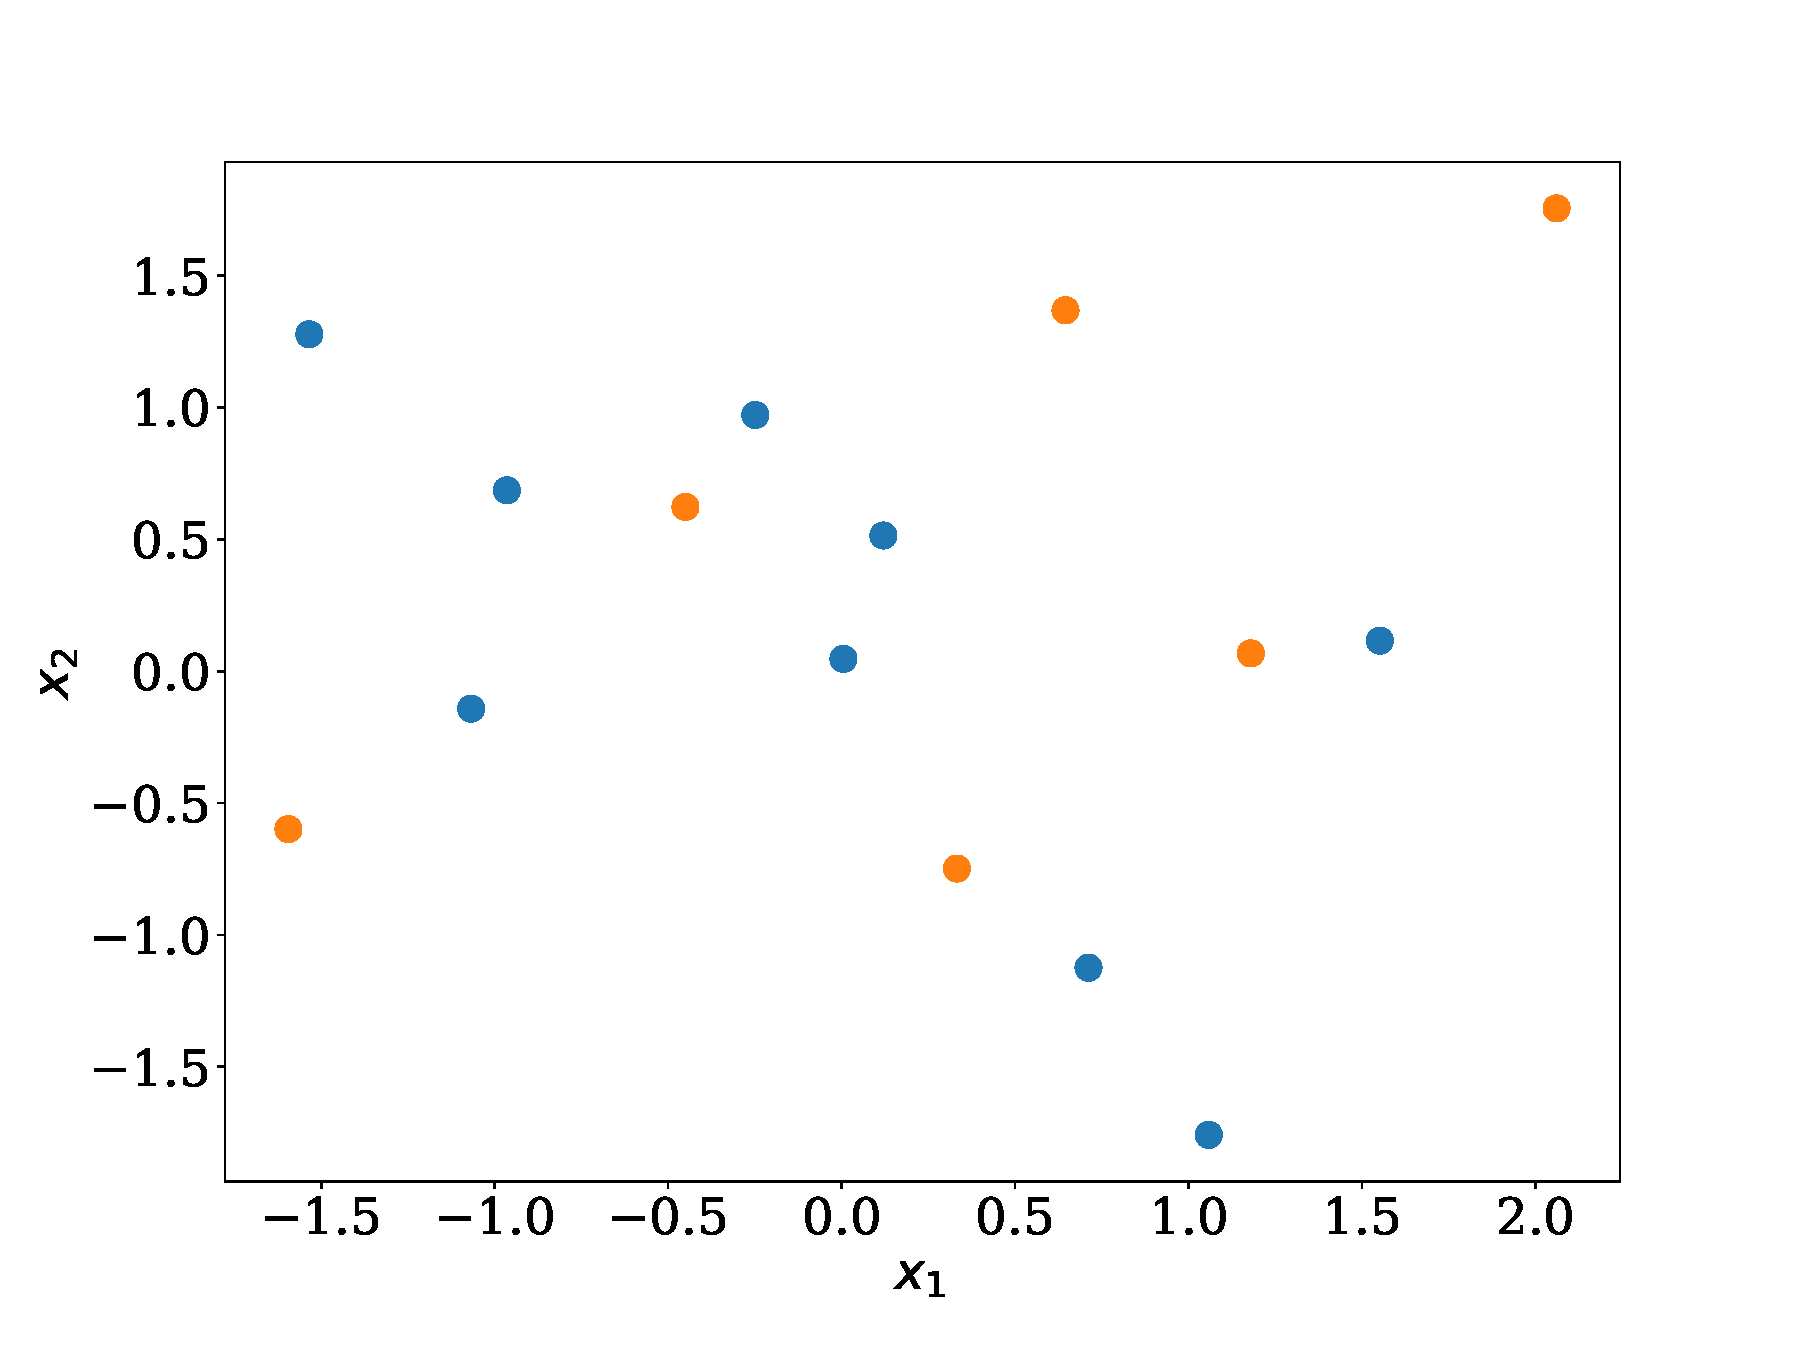
\includegraphics[width=\linewidth]{train.pdf}
    \caption{}}
    \end{subfigure}
    \begin{subfigure}[h]{0.325\linewidth}
    \center{
    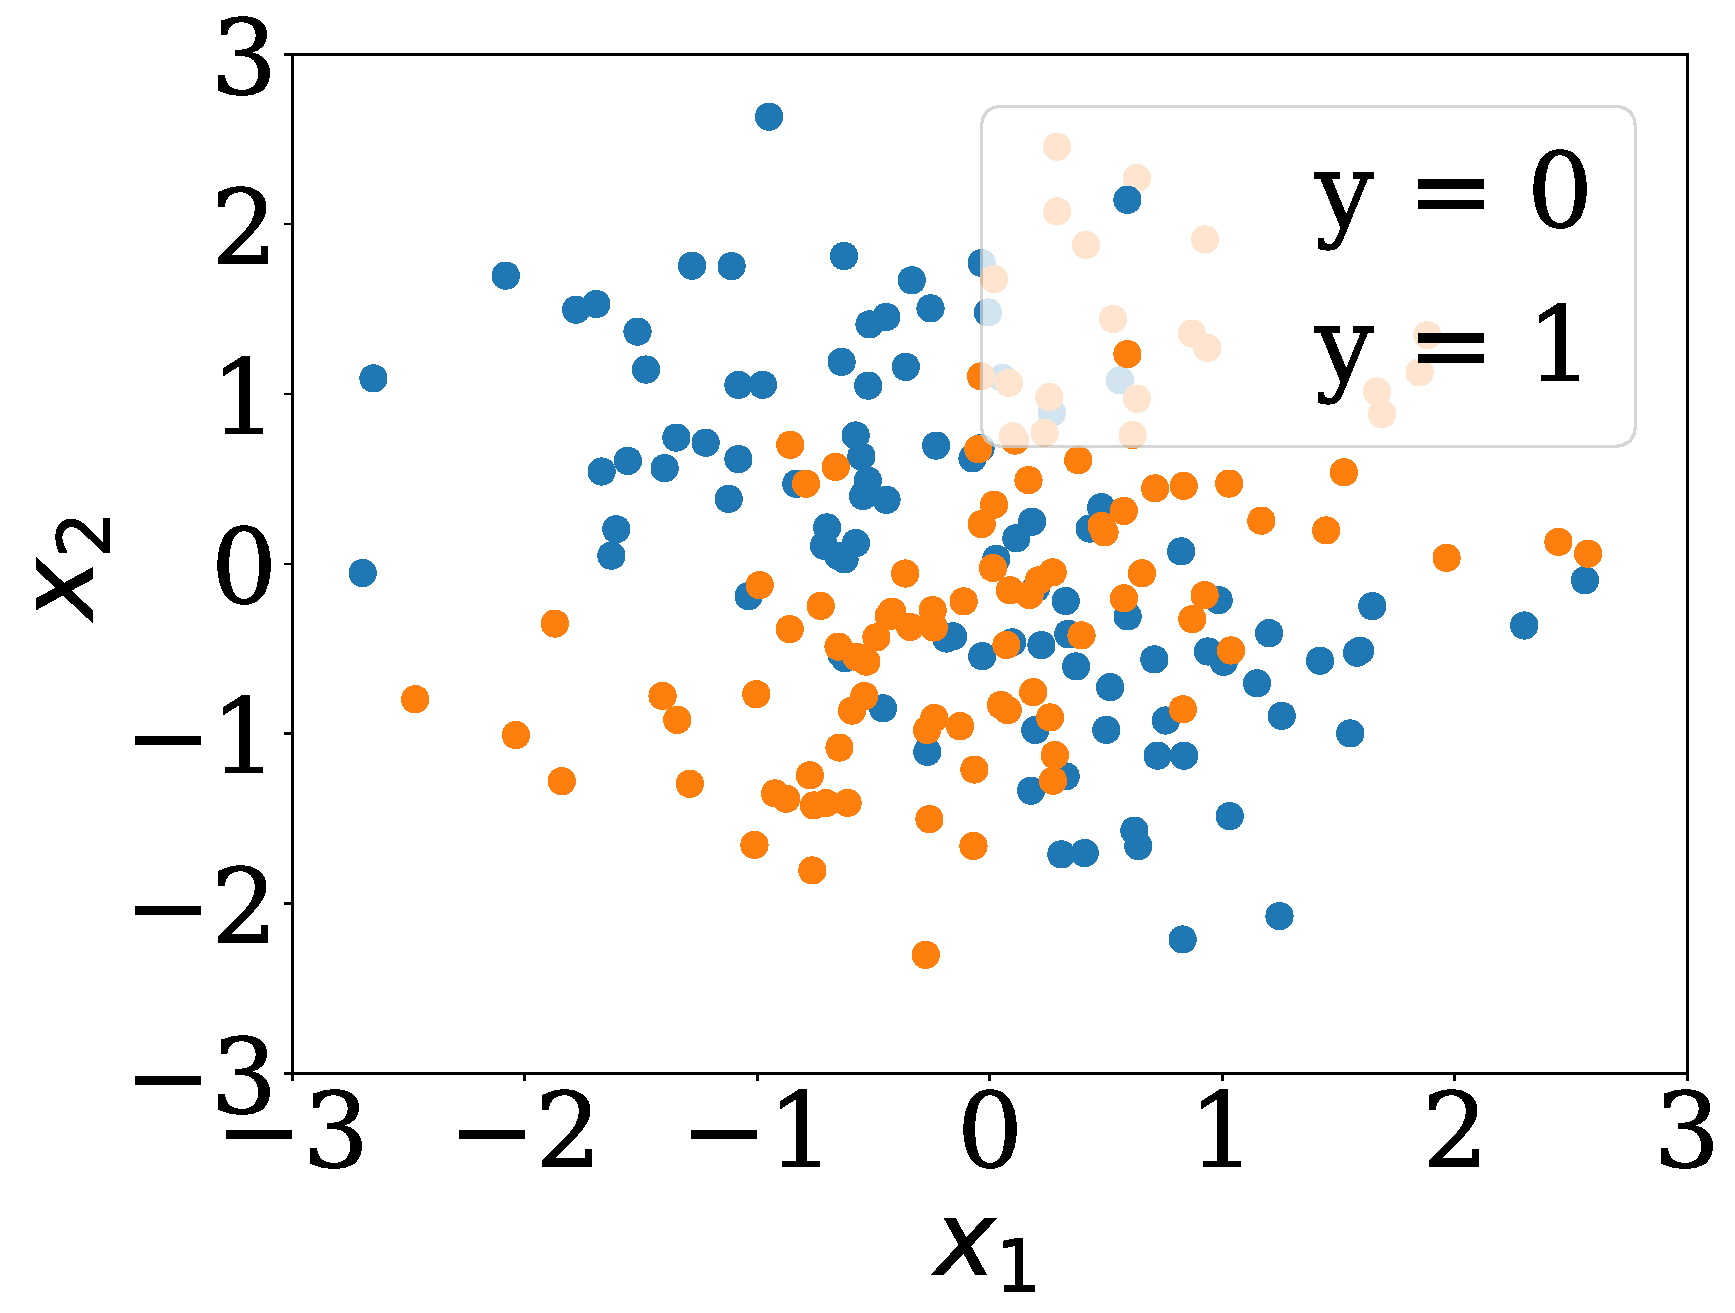
\includegraphics[width=\linewidth]{test.pdf}
    \caption{}}
    \end{subfigure}
    
    % \vspace{-0.2 cm}
    
    \caption{%\fontsize{8}{5}\selectfont
    Visualization of a) teacher model dataset; b) student model dataset; c) test part}
    \label{fig:synth}
\end{figure}


\begin{figure}[ht]
    \begin{subfigure}[h]{0.5\linewidth}
    \center{
    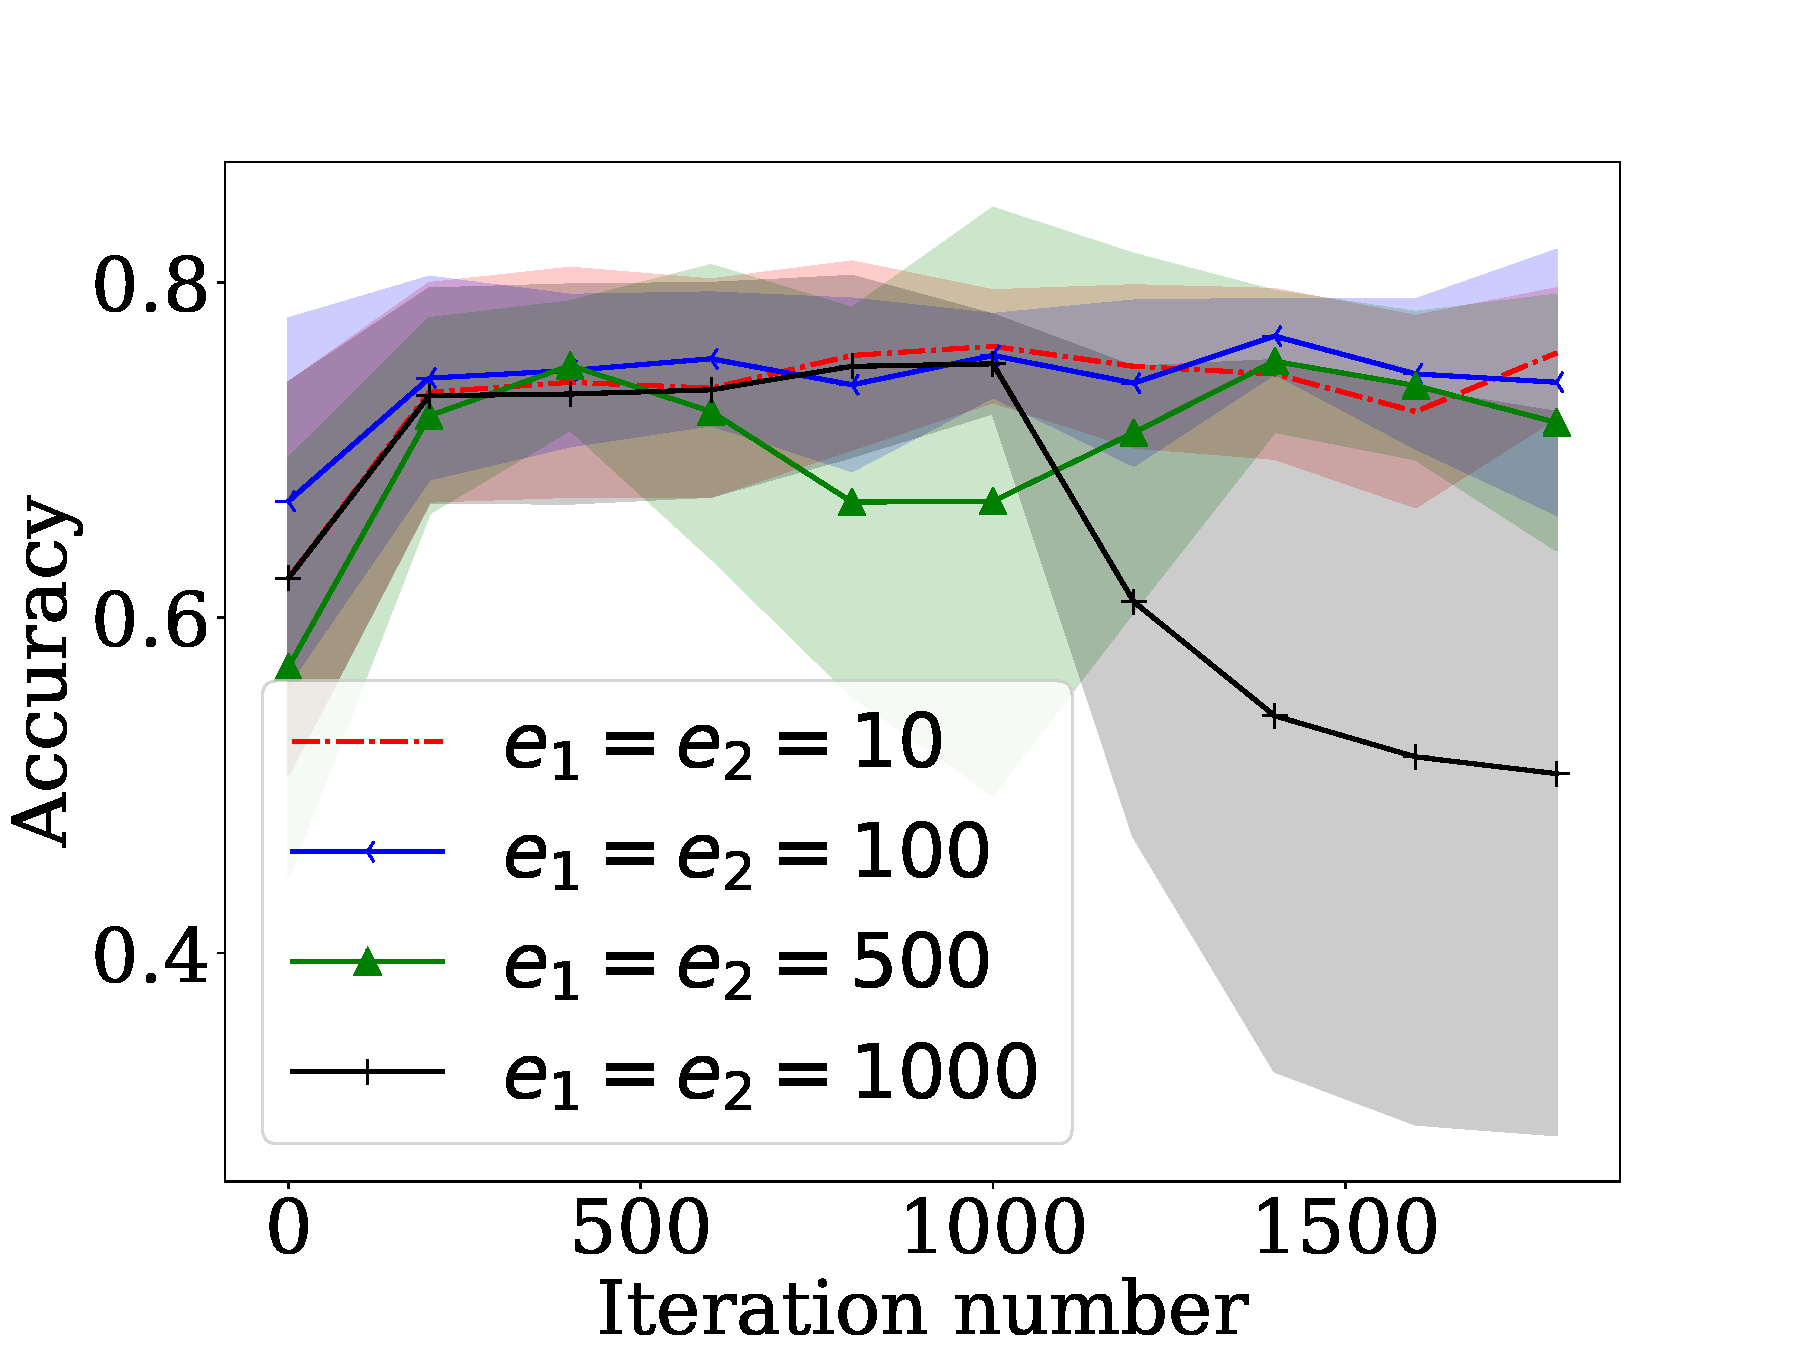
\includegraphics[width=\linewidth]{synth_mini_epoch_size.pdf}}
    \caption{}
    \label{fig:epoch_size}
    \end{subfigure}
    \begin{subfigure}[h]{0.5\linewidth}
    \center{
    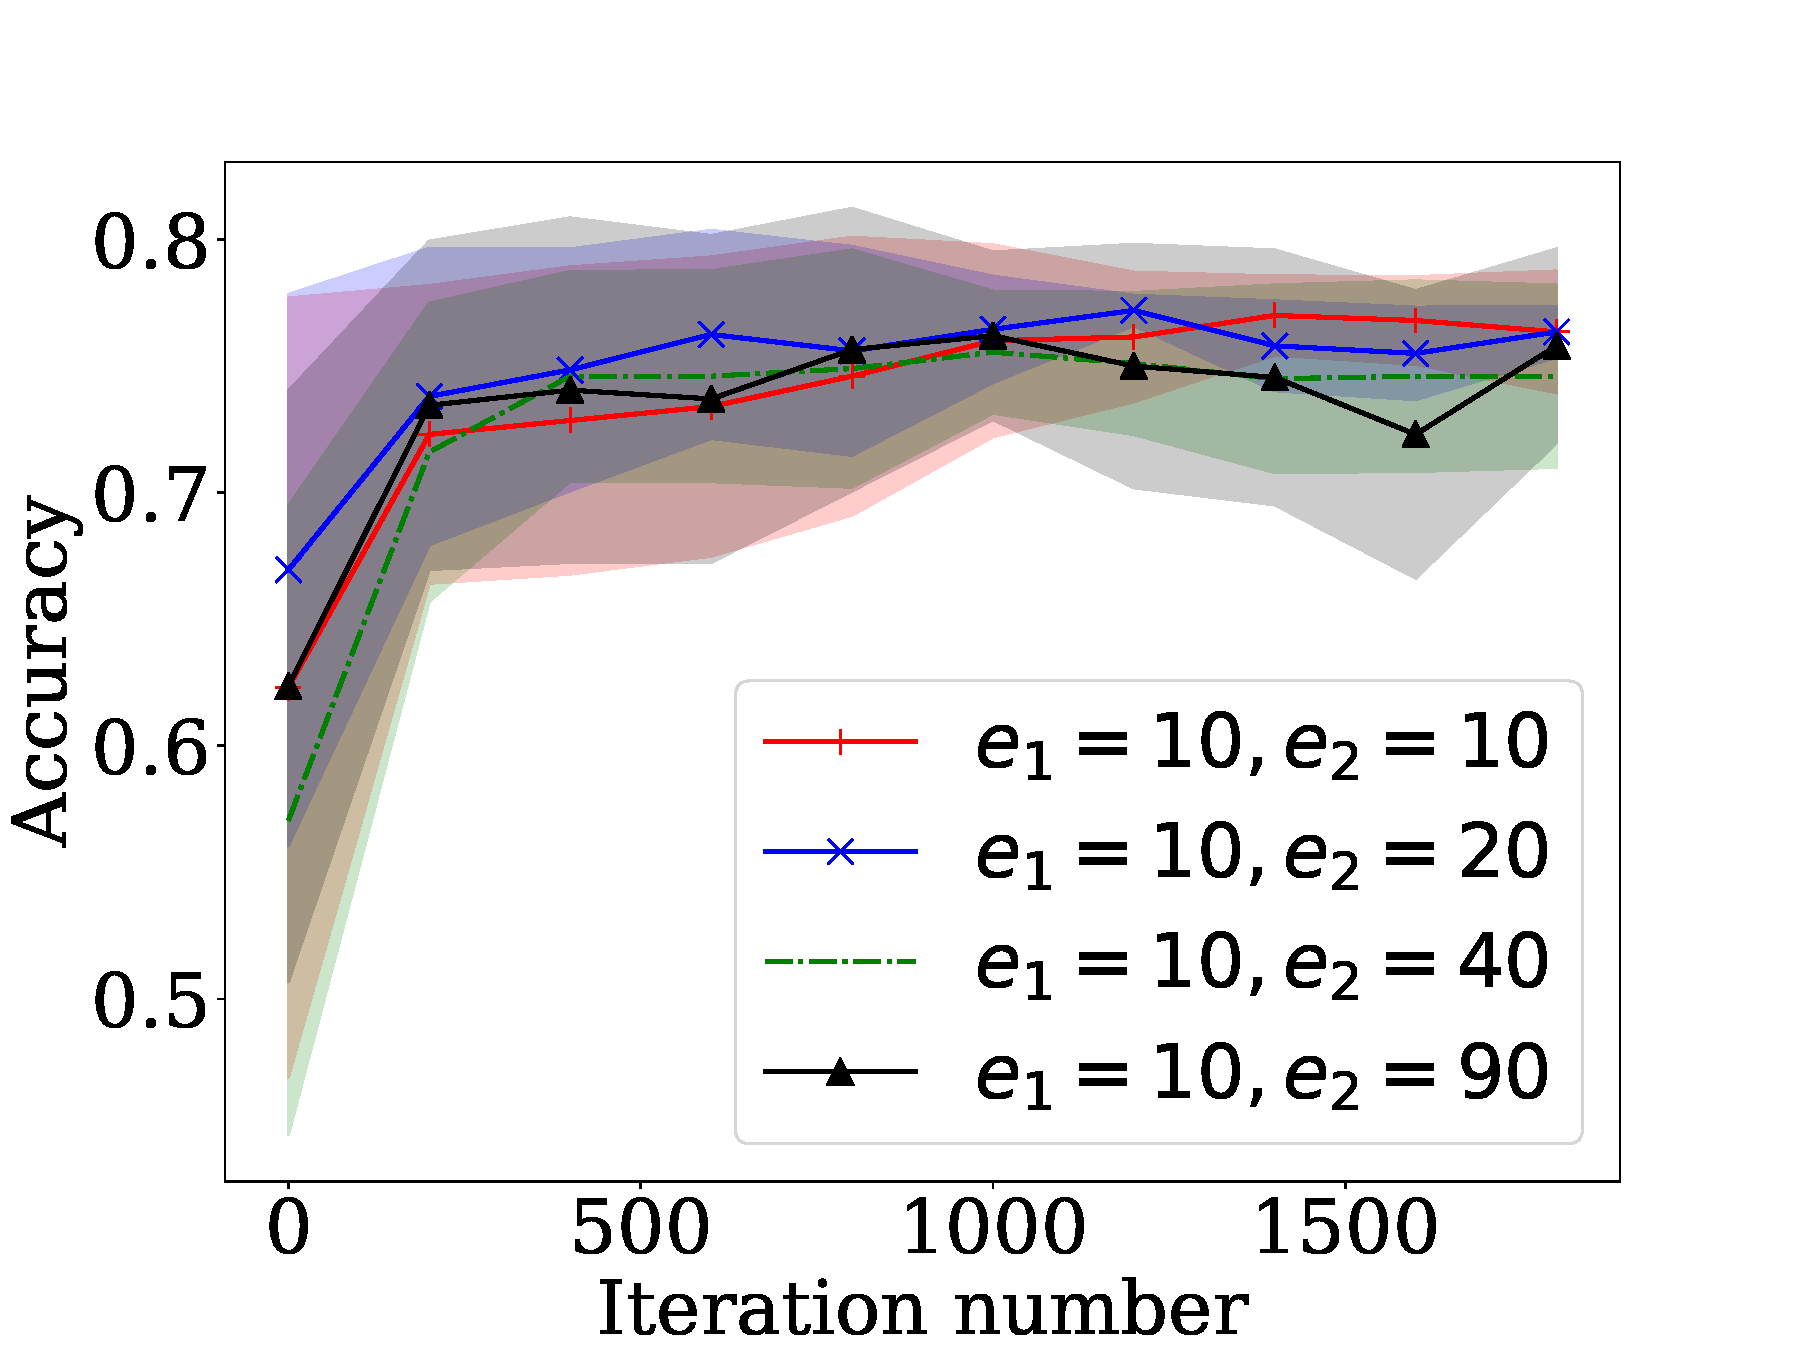
\includegraphics[width=\linewidth]{synth_period.pdf}}
    \caption{}
    \label{fig:train_splines_every_epoch}
    \end{subfigure}
    % \vspace{-0.2 cm}
    \caption{%\fontsize{10}{5}\selectfont
    Model accuracy with $e_1$ and $e_2$ values: a) $e_1 = e_2$; b) variation of $e_2$ with $e_1 =10$.}
    \label{fig:epoch_size}
\end{figure}
 

Fig. \ref{fig:accuracy}.a plots model accuracy for different methods. The best results were obtained with optimized metaparameters and the proposed method. As we can see, the proposed method gives a good approximation for the metaparameter optimization for this experiment.



\subsection{Experiments on CIFAR-10 and Fashion-MNIST datasets}
We split both the dataset in the ratio 9:1 for the training and validation.  For the model parameter optimization, we used stochastic gradient descent with initial learning set to 1.0. The learning rate was multiplied by 0.5 every 10 epochs. We set  $T_\text{val}$ equal to 1.0.

For the experiments on CIFAR-10 we used the pretrained ResNet model from~\cite{pkt_eccv} as a teacher. As a student, we used CNN model with three convolutional layers and two fully connected layers. 
For the experiments on the reduced dataset, we used the learning rate for the metaparameter optimization equal to 0.25 and trained the model for 50 epochs. For  the experiments on the full dataset, we used  the learning rate for the metaparameters set to 0.1. We trained the model for 100 epochs. 

For the experiments on Fashion-MNIST, we used teacher and student model architectures similar to those in CIFAR-10 experiments. We used the learning rate for the metaparameter optimization equal to 0.1 and trained the model for 50 epochs.

As we can see from the results from the Table~\ref{table:results}, the both the proposed method and gradient-based method give quite competitive results. The probabilistic model-based method shows a similar performance. Thus, the gradient-based methods are preferable because they have similar performance but require fewer optimization iterations. At the same time, the gradient-based methods suffer from getting stuck in local minima, so the variance of their results is much higher than that of other methods. This can be seen from the Fig.~\ref{fig:accuracy} and the Table~\ref{table:results}.

\section{Conclusion}
The parameter optimization problem for deep learning models was analyzed. The generalization of knowledge distillation method was proposed that uses gradient-based metaparameter optimization. Model parameters are optimized on the first level and metaparameters on the second. We proposed a method to reduce metaparameter optimization cost for gradient-based optimization. The proposed method  was evaluated in the numerical experiment on the Fashion-MNIST, CIFAR-10 datasets and on the synthetic dataset. The computational experiment showed the effectiveness of gradient-based optimization for selecting of metaparameters of the distillation loss function. The possibility of optimization path approximation using linear models was analyzed. In future, we are planning to investigate more complicated predictive models for  metaparameter optimization. 

% Please note that the first paragraph of a section or subsection is
% not indented. The first paragraph that follows a table, figure,
% equation etc. does not need an indent, either.

% Subsequent paragraphs, however, are indented.

% \subsubsection{Sample Heading (Third Level)} Only two levels of
% headings should be numbered. Lower level headings remain unnumbered;
% they are formatted as run-in headings.

% \paragraph{Sample Heading (Fourth Level)}
% The contribution should contain no more than four levels of
% headings. Table~\ref{tab1} gives a summary of all heading levels.

% \begin{table}
% \caption{Table captions should be placed above the
% tables.}\label{tab1}
% \begin{tabular}{|l|l|l|}
% \hline
% Heading level &  Example & Font size and style\\
% \hline
% Title (centered) &  {\Large\bfseries Lecture Notes} & 14 point, bold\\
% 1st-level heading &  {\large\bfseries 1 Introduction} & 12 point, bold\\
% 2nd-level heading & {\bfseries 2.1 Printing Area} & 10 point, bold\\
% 3rd-level heading & {\bfseries Run-in Heading in Bold.} Text follows & 10 point, bold\\
% 4th-level heading & {\itshape Lowest Level Heading.} Text follows & 10 point, italic\\
% \hline
% \end{tabular}
% \end{table}


% \noindent Displayed equations are centered and set on a separate
% line.
% \begin{equation}
% x + y = z
% \end{equation}
% Please try to avoid rasterized images for line-art diagrams and
% schemas. Whenever possible, use vector graphics instead (see
% Fig.~\ref{fig1}).

% \begin{figure}
% \includegraphics[width=\textwidth]{fig1.eps}
% \caption{A figure caption is always placed below the illustration.
% Please note that short captions are centered, while long ones are
% justified by the macro package automatically.} \label{fig1}
% \end{figure}

% \begin{theorem}
% This is a sample theorem. The run-in heading is set in bold, while
% the following text appears in italics. Definitions, lemmas,
% propositions, and corollaries are styled the same way.
% \end{theorem}
%
% the environments 'definition', 'lemma', 'proposition', 'corollary',
% 'remark', and 'example' are defined in the LLNCS documentclass as well.
%
% \begin{proof}
% Proofs, examples, and remarks have the initial word in italics,
% while the following text appears in normal font.
% \end{proof}
% For citations of references, we prefer the use of square brackets
% and consecutive numbers. Citations using labels or the author/year
% convention are also acceptable. The following bibliography provides
% a sample reference list with entries for journal
% articles~\cite{ref_article1}, an LNCS chapter~\cite{ref_lncs1}, a
% book~\cite{ref_book1}, proceedings without editors~\cite{ref_proc1},
% and a homepage~\cite{ref_url1}. Multiple citations are grouped
% \cite{ref_article1,ref_lncs1,ref_book1},
% \cite{ref_article1,ref_book1,ref_proc1,ref_url1}.
%
% ---- Bibliography ----
%
% BibTeX users should specify bibliography style 'splncs04'.
% References will then be sorted and formatted in the correct style.
%

%
% \begin{thebibliography}
\bibliographystyle{splncs04.bst}
% \nocite{*}
\bibliography{bibliography.bib}
% \bibitem{ref_article1}
% Author, F.: Article title. Journal \textbf{2}(5), 99--110 (2016)

% \bibitem{ref_lncs1}
% Author, F., Author, S.: Title of a proceedings paper. In: Editor,
% F., Editor, S. (eds.) CONFERENCE 2016, LNCS, vol. 9999, pp. 1--13.
% Springer, Heidelberg (2016). \doi{10.10007/1234567890}

% \bibitem{ref_book1}
% Author, F., Author, S., Author, T.: Book title. 2nd edn. Publisher,
% Location (1999)

% \bibitem{ref_proc1}
% Author, A.-B.: Contribution title. In: 9th International Proceedings
% on Proceedings, pp. 1--2. Publisher, Location (2010)

% \bibitem{ref_url1}
% LNCS Homepage, \url{http://www.springer.com/lncs}. Last accessed 4
% Oct 2017
% \end{thebibliography}
\end{document}
